\documentclass{beamer}
\DeclareFontShape{OT1}{cmss}{b}{n}{<->ssub * cmss/bx/n}{} 
\usetheme{default}
\usepackage{amsmath}
\usepackage{amsfonts}
\usepackage{mathbbol}
\usepackage{xcolor} % before tikz or tkz-euclide if necessary
\usepackage{tkz-euclide} % no need to load TikZ
\usepackage{multirow}
\usepackage{lmodern}
\usepackage{bm}

\title{Statistical Machine Learning\\ Part 7\\
Tree-Based Methods}
\author{Horacio G\'omez-Acevedo\\ Department of Biomedical Informatics\\
University of Arkansas for Medical Sciences}
\begin{document}
	\begin{frame}[plain]
		\maketitle
	\end{frame}
	
	
	\begin{frame}{Tree structures}
		
		A typical tree is depicted with the root being the top node, and growing down. Decisions are being made at each node until a terminal node or {\it leaf} is reached. Each non-terminal node contains a question on which a split is based. Each leaf contains the label (classification) or the predicted mean value (regression).
		 
		
		
\end{frame}

\begin{frame}{Regression Trees}

We will use the {\bf Hitters} data set as an example for  regression.  After running the code we obtain the following figure

\begin{figure}[h]
	\centering
	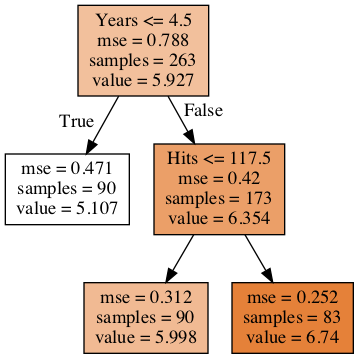
\includegraphics[scale=0.5]{../../Figures/fig_hitters.png}
\end{figure}
	
	
\end{frame}

\begin{frame}{Regression Trees (cont)}
	How to read this information?
	The main feature for this set is {\it years}, from which the total samples are split into two depending on whether their time spent in the baseball league has been less than 4.5 years. The case on the left (True) is already given a value of $5.107$, which means that the average salary is $\exp(5.107)\approx 165.17$ thousand dollars a year. Players with more than 4.5 years will be further divided into the variable ${\it hits} $, and someone above 117.5 will earn on average $\exp(6.74)=845.56$ thousand dollars!
\end{frame}

\begin{frame}{Regression Trees (cont)}
	We can see that the graphical representation of a tree is as follows
	
	\begin{figure}[h]
		\centering
		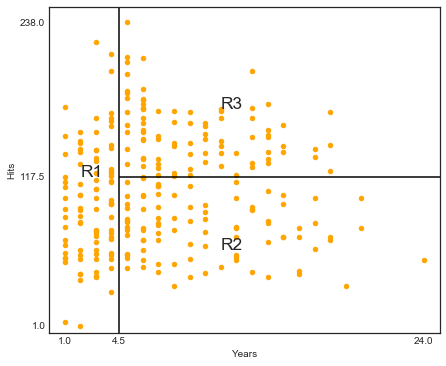
\includegraphics[scale=0.5]{../../Figures/fig_hitters_graph.png}
	\end{figure}
The regions $R_i$ are the representing the leaves of the tree.  	
	
\end{frame}

\begin{frame}{Prediction in Regression Trees}
	There are two main steps involved in building a tree
	
	\begin{itemize}
		\item Divide the predictor space $X_1 \times X_2 \times \cdots \times X_p$ into $J$ distinct and non-overlapping regions $R_1,\ldots, R_J$.
		\item For every observation that falls into the region $R_j$, we make the same prediction, which is the mean of the response values for the training observations in $R_j$.
	\end{itemize}
\end{frame}

\begin{frame}{2D Example}
	Suppose we have the outcome $Z$ depending on two predictors $X$ and $Y$ defined in certain rectangular area $A\subset X \times Y$ of the plane. One feasible partition of $A$ is depicted below
		\begin{figure}[h]
		\centering
		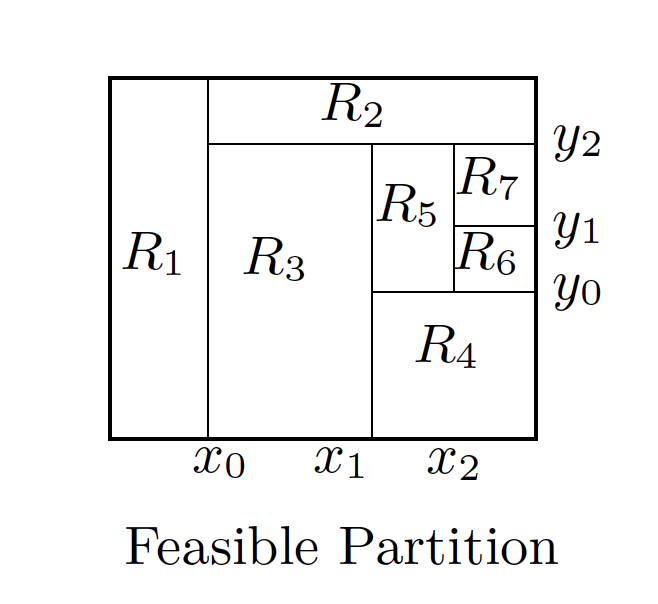
\includegraphics[scale=0.5]{../../Figures/fig_tree_region.png}
	\end{figure}
	
\end{frame}

\begin{frame}{2D Example (cont)}
The previous partition can be described as a tree structure
\begin{figure}[h]
	\centering
	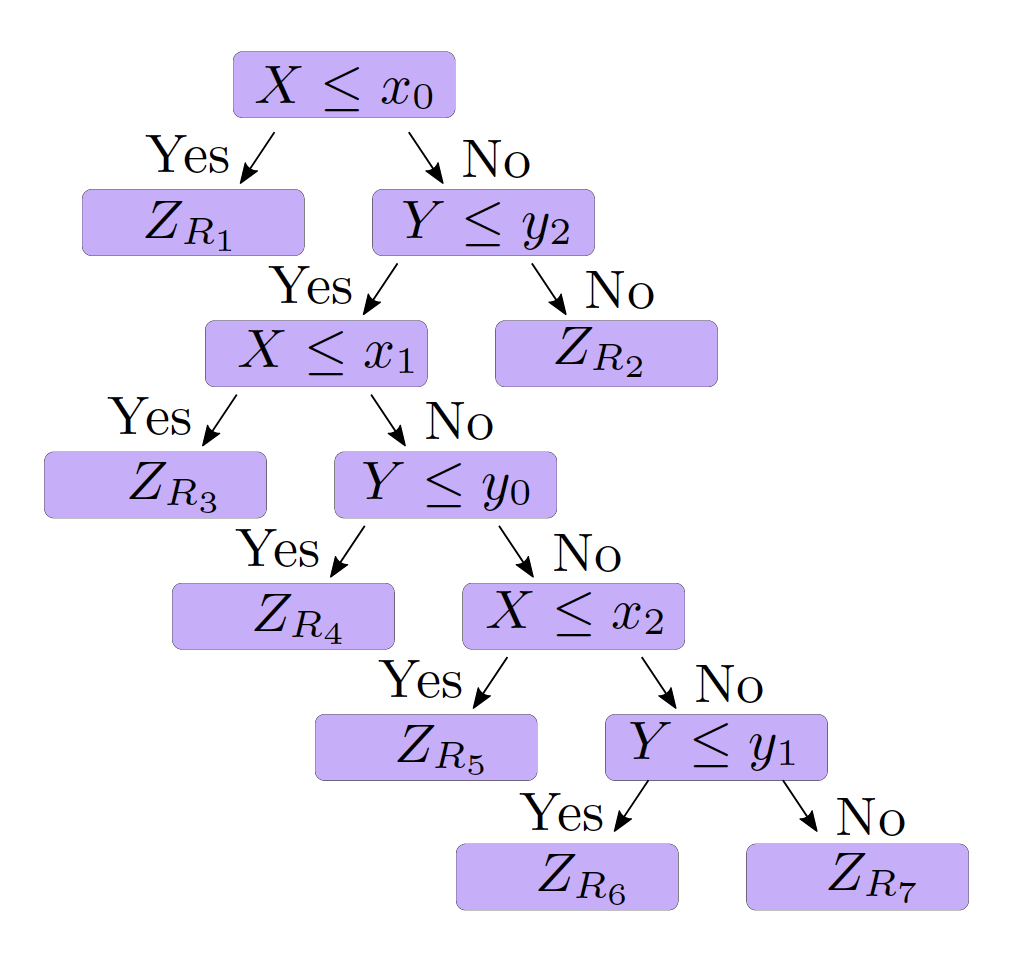
\includegraphics[scale=0.3]{../../Figures/fig_tree_trans.png}
\end{figure}

The corresponding prediction for $\widehat{Z}(x,y)$ based on given partition of $A$ is defined as 
\begin{equation*}
	\widehat{Z}(x,y)= \textrm{Average} \{ Z(x_r,y_r)\colon (x_r ,y_r)\in R_j)\}
\end{equation*}
where $(x,y) \in R_j$.

\end{frame}

\begin{frame}{References}

Materials and some of the pictures are from (1),(2), and (3).
\begin{enumerate}
	\item Gareth James et al. {\it An Introduction to Statistical Learning with applications in R}. Springer (2015)
	\item Richard O. Duda et al. {\it Pattern Classification} John Wiley (2001). 
	\item Aur\'elien G\'eron. {\it Hands-on Machine Learning with Scikit-Learn \& TensorFlow} O'Relly (2017)
	\item Wiebe R. Pestman {\it Mathematical Statistics} de Gruyter (1998)
	\item Bradley Efron. {\it The Jackknife, the Bootstrap and other Resampling Plans}  SIAM (1982)
	\item Bradley Efron {\it A 250-year argument: Belief, behavior and the bootstrap} Bull. Am. Math. Soc (2012)
\end{enumerate}	

I have used some of the graphs by hacking TiKz code from StakExchange, Inkscape for more aesthetic plots and other old tricks of \TeX
\end{frame}	


\end{document}
